\documentclass[conference]{IEEEtran}

\IEEEoverridecommandlockouts
% The preceding line is only needed to identify funding in the first footnote. If that is unneeded, please comment it out.
\usepackage{cite}
\usepackage{amsmath,amssymb,amsfonts}
\usepackage{algorithmic}
\usepackage{graphicx}
\usepackage{textcomp}
\usepackage{xcolor}
\def\BibTeX{{\rm B\kern-.05em{\sc i\kern-.025em b}\kern-.08em
    T\kern-.1667em\lower.7ex\hbox{E}\kern-.125emX}}
\begin{document}

\title{Coordinated Voltage Control in Distribution
Systems with Distributed Generations}

\author{\IEEEauthorblockN{Alvi Newaz}
\IEEEauthorblockA{Electrical and Computer Engineering\\
Florida State University\\
Tallahassee, Florida\\
Email: an15m@fsu.edu}
\and
\IEEEauthorblockN{Juan Ospina} 
\IEEEauthorblockA{Electrical and Computer Engineering\\
Florida State University\\
Tallahassee, Florida\\
Email: jjospina@fsu.edu}
\and
\IEEEauthorblockN{M. Omar Faruque} 
\IEEEauthorblockA{Electrical and Computer Engineering\\
Florida State University\\
Tallahassee, Florida\\
Email: faruque@caps.fsu.edu}

}

\maketitle

\graphicspath{{figs/}}
\begin{abstract}
This paper presents a centralized coordinated voltage control algorithm for distribution systems with distributed generations (DGs).  The control algorithm coordinates the use of available distributed generation (DG) with the traditional voltage regulation devices, taking into consideration the reactive power limits of the DG inverters to maintain the system voltage within predefined limits. With the help of the developed algorithm the  reactive power generation capacity of the DG inverters can be used to cope with the dynamic generation of the DGs without increasing the operations of the traditional voltage regulation devices available.
\end{abstract}

\begin{IEEEkeywords}
Distributed generations, voltage regulation devices, Coordinated Voltage Control
\end{IEEEkeywords}

\section{Introduction}\label{sec:intro}
The energy industry is rapidly approaching a significant penetration of distributed generation (DG) in the distribution system. This higher penetration of distributed energy resources (DERs) has introduced reverse power flow in the system. The traditional voltage regulation devices only consider unidirectional power flow and operate based on the consideration that the voltage down the line will decrease depending on the line impedance. But this assumption is not valid with distributed generation as they can change the voltage of a node by supplying or absorbing reactive power. The uncertainty of the distributed wind and solar renewable resources can also cause traditional voltage regulation devices to operate more than necessary \cite{int1}.

With the rise of technology such as smart grid, advanced metering infrastructure (AMI) and phasor measurement units (PMUs), a lot more data regarding the system status is available. How to efficiently use this data to optimize the voltage control coordination is still a contemporary research topic. In most of the current literature, this problem is addressed as an optimum power flow problem or a mixed integer optimization problem \cite{int2}. But both these approaches usually propose methods which are very computationally intensive and time consuming. For example, in \cite{LR5,LR1,LR2,LR3}, researchers describe various methods to coordinate voltage control using the DG and traditional voltage regulation devices. But the control cycles in these methods are in the range of minutes to an hour \cite{LR4}. This makes them unfavorable for controlling the voltage in a distribution grids containing fast responding DGs.

This paper proposes a coordinated voltage control method that reduces the use of traditional voltage control devices and utilizes the reactive power generation capabilities of the DG inverters to regulate the distribution system voltage. The proposed algorithm enables cooperation between multiple DGs to control the system voltage. This ensures that the full potential of the DG inverters is utilized before using the traditional devices for voltage regulation. The proposed method also completes its control cycle within a second which makes it suitable for distribution grids containing fast changing DGs. The proposed method has been validated using a distribution feeder model based on a real feeder. A phasor model of the system with the control algorithm was simulated in MATLAB\textsuperscript{\textregistered} Simulink\textsuperscript{\textregistered} using the Simscape Power Systems\textsuperscript{TM} toolbox for validation.

The rest of the paper is organized as follows. Section II contains the theoretical background and the proposed algorithm. Section III contains the details about the test feeder. Section IV contains the validation and results while Section VI includes the concluding remarks.

\section{Design of Control Algorithm}\label{sec:design}
The proposed algorithm makes use of two concepts to coordinate the voltage regulation between the nodes. They are:
\begin{itemize}
\item Voltage sensitivity analysis
\item Electrical distance calculation
\end{itemize}

\subsection{Voltage Sensitivity Analysis}
The aim of the voltage sensitivity analysis is to determine the effect on the voltage due to reactive power injection at different nodes. Equation (\ref{eq.Pf_equation}) represents the system power-flow equation.  Here ${\Delta Q}, {\Delta P}, {\Delta |V|}$ and ${\Delta \delta}$ represent the change in real power, reactive power, voltage magnitude and voltage angle of nodes. $J$ represents the system jacobian matrix. The elements of $J$ are shown in (\ref{eq.J_equation})
\begin{equation}\label{eq.Pf_equation}
\begin{bmatrix}
{\Delta P}\\ {\Delta Q}
\end{bmatrix} =J\begin{bmatrix}
{\Delta|V|} \\ {\Delta\delta}
\end{bmatrix}
\end{equation}  
Where,
\begin{equation}\label{eq.J_equation}
    J = \begin{bmatrix}
{J_{P|V|}} & {J_{P\delta}}\\ {J_{Q|V|}} & {J_{Q\delta}}
\end{bmatrix}
\end{equation}

Using the components of the system Jacobian matrix the $J_{VQ}$ and $J_{VP}$ matrices can be formulated using (\ref{eq.JVQ}) and (\ref{eq.JVP}).
\begin{equation}\label{eq.JVQ}
    {J_{VQ}} = {J_{Q|V|}}-{J_{Q\delta}}{J_{P\delta}}^{-1}{J_{P|V|}}
\end{equation}

\begin{equation}\label{eq.JVP}
    {J_{VP}}={J_{P|V|}}-{J_{P\delta}}{J_{Q\delta}}^{-1}{J_{Q|V|}}
\end{equation}

Using (\ref{eq.JVQ}) and (\ref{eq.JVP}) the total voltage sensitivity due to real and reactive power injected by a DG can be calculated using (\ref{eq.V_PQ}) \cite{Th_ali}. Here, $[\Delta|V|_{PQ}] , [P_{PV}] $ and $[Q_{PV}]$ represent the total voltage change, real power injected by DG and reactive power injected by DG respectively.

\begin{equation}\label{eq.V_PQ}
[\Delta|V|_{PQ}] ={ J_{VP}}^{-1} [P_{PV}]+{ J_{VQ}}^{-1} [Q_{PV}]
\end{equation}

Using the relation $[P_{PV}] = \frac{[Q_{PV}]}{\cos^{-1}(p.f)}$ equation (\ref{eq.V_PQ}) can be written as
\begin{equation}\label{eq.V_Q}
 [\Delta|V|_{PQ}] ={ J_{VP}}^{-1}\frac{[Q_{PV}]}{\cos^{-1}(p.f)} +{ J_{VQ}}^{-1} [Q_{PV}]
\end{equation}
 Equation (\ref{eq.V_Q}) gives us the relation between total voltage sensitivity and reactive power injection. Here, '$p.f$' represents power factor.

\subsection{Electrical Distance Calculation}
Electrical distance is calculated in order to determine the relative impact on one node due to change in another node. The electrical distances are calculated by determining $M_{sVQ}$ according to equation (\ref{MsQV}) \cite{int1}.

\begin{equation}\label{MsQV}
\begin{bmatrix}
M_{s\alpha}P & M_{s\alpha}Q \\ 
M_{sVP} & M_{sVQ} 
\end{bmatrix} = J^{-1}
\end{equation}
 Here, $J$ is the system jacobian matrix and $M_{s\alpha}P, M_{s\alpha}Q, M_{sVP}$ and $M_{sVQ}$  are the four elements of the inverse of the system jacobian matrix. Equation (\ref{MsVq_expan}) shows the elements of $M_{sVQ}$. \cite{int1}

\begin{equation}\label{MsVq_expan}
M_{sVQ} =
\begin{bmatrix}
\frac{\delta V_{s1}}{\delta Q_{s1}}  & \frac{\delta V_{s1}}{\delta Q_{s2}} & \cdots & \frac{\delta V_{s1}}{\delta Q_{sn}}\\

\frac{\delta V_{s2}}{\delta Q_{s1}}  & \frac{\delta V_{s2}}{\delta Q_{s2}} & \cdots & \frac{\delta V_{s2}}{\delta Q_{sn}}\\

\vdots & \vdots & \vdots & \vdots\\

\frac{\delta V_{sn}}{\delta Q_{s1}}  & \frac{\delta V_{sn}}{\delta Q_{s2}} & \cdots & \frac{\delta V_{sn}}{\delta Q_{sn}}\\ 
\end{bmatrix}
\end{equation}
 
Here $V_{sn}$ and $Q_{sn}$ represent the voltage and reactive power of the node $n$. The electrical distance $D_{sij}$ between the nodes $i$ and $j$ can be calculated using (\ref{ED}) \cite{int1}. 

\begin{equation}\label{ED}
D_{sij} = -\log (\mu_{sij} * \mu_{sji})
\end{equation}

Where,
$$
\mu_{sij} =  \frac{\delta V_{si}}{\delta Q_{sj}} / \frac{\delta V_{sj}}{\delta Q_{sj}}
$$
After determining the electrical distances the nodes are separated into different zones to determine which DG should provide reactive power support for voltage control.

\subsection{Singular value decomposition and pseudo inverse}
In case of a distribution system the system jacobian matrix $J$ is usually a sparse matrix due to the radial nature of distribution systems. Calculating the inverse of $J$ becomes problematic due to this property. For this reason (\ref{eq.V_Q}) and (\ref{ED}) are implemented by determining the pseudo inverse of $J$ using singular value decomposition. The system jacobian matrix $J$ can factored into the expression shown in (\ref{eq.SVD}) \cite{PINV}.
\begin{equation}\label{eq.SVD}
    J = USV^T
\end{equation}

Here, $U$ is an orthogonal matrix whose columns are the eigenvectors of $JJ^T$. $V$ is another orthogonal matrix whose columns are the  eigenvectors of $J^{T}J$. $S$ is a diagonal matrix and is the same size as $J$. Its diagonal elements are the square roots of the nonzero eigenvalues of both $JJ^T$ and $J^{T}J$. The elements of $S$ are the singular values of $J$ and they are represented as $\sigma_1, \sigma_2, ..., \sigma_r$ where $r$ is the rank of $J$. After factoring $J$ into these three components the pseudo inverse of $J$, $J^+$ can be calculated using (\ref{eq.PINV}) \cite{PINV}
\begin{equation}\label{eq.PINV}
    J^+ = US^{+}V^T
\end{equation}
$S^+$ is calculated by taking the reciprocal of all the non-zero elements of $S$ and leaving all the zero elements alone \cite{PINV}.  

\subsection{Control Algorithm}
The core functionality of the algorithm proposed is based on the voltage sensitivity analysis and the concept of electrical distances calculation mentioned before. The main objective of the coordinated voltage control algorithm is the monitoring and control of the voltage at each node of the system, by using inverter-based reactive power and voltage control with traditional voltage regulation devices in order to keep the voltages between the range desired. The calculation of the reactive power needed to be injected is obtained by using the voltage sensitivity and electrical distances concepts. The main steps of the control algorithm is given below.

\begin{enumerate}
%1
\item \textbf{Identify the nodes with voltage limit violation from measured data}
%2
\item \textbf{Determine node with highest voltage deviation.}
%3
\item \textbf{Construct system Jacobian matrix}
%4
\item \textbf{Calculate voltage sensitivity matrix}
%5
\item \textbf{Calculate electrical distances}
%6
\item \textbf{Order the nodes:} In this step, the nodes capable of providing reactive power support are ordered according to their electrical distance from the selected affected node. The ordered list of nodes is saved in a list called \textit{Node\_list}
%7
\item \textbf{Apply the appropriate reactive power:} In this step, the first node in the \textit{Node\_list} is selected. If the node has the capability to supply the required reactive power determined by the sensitivity matrix the algorithm sets the node to provide the required amount of power and continues to \textbf{step 9}. Otherwise, the algorithm sets the node to deliver the maximum available reactive power and takes it out of the list of nodes capable of providing reactive power.
%8
\item \textbf{Repeat steps 3 to 7}
%9
\item \textbf{Estimate new system status:} After deciding the change in node reactive powers the algorithm estimates the new voltage profile of the system using (\ref{eq.Q_V}). If all the nodes in the new estimated profile are within voltage limits the algorithm continues to \textbf{step 10}. Otherwise the algorithm updates the measured data collected from the system with the new estimates and goes back to  \textbf{step 1}.

%10
\item \textbf{Request the devices at the nodes to apply calculated changes}
\end{enumerate}

% \begin{figure}[h]
% \centering
% 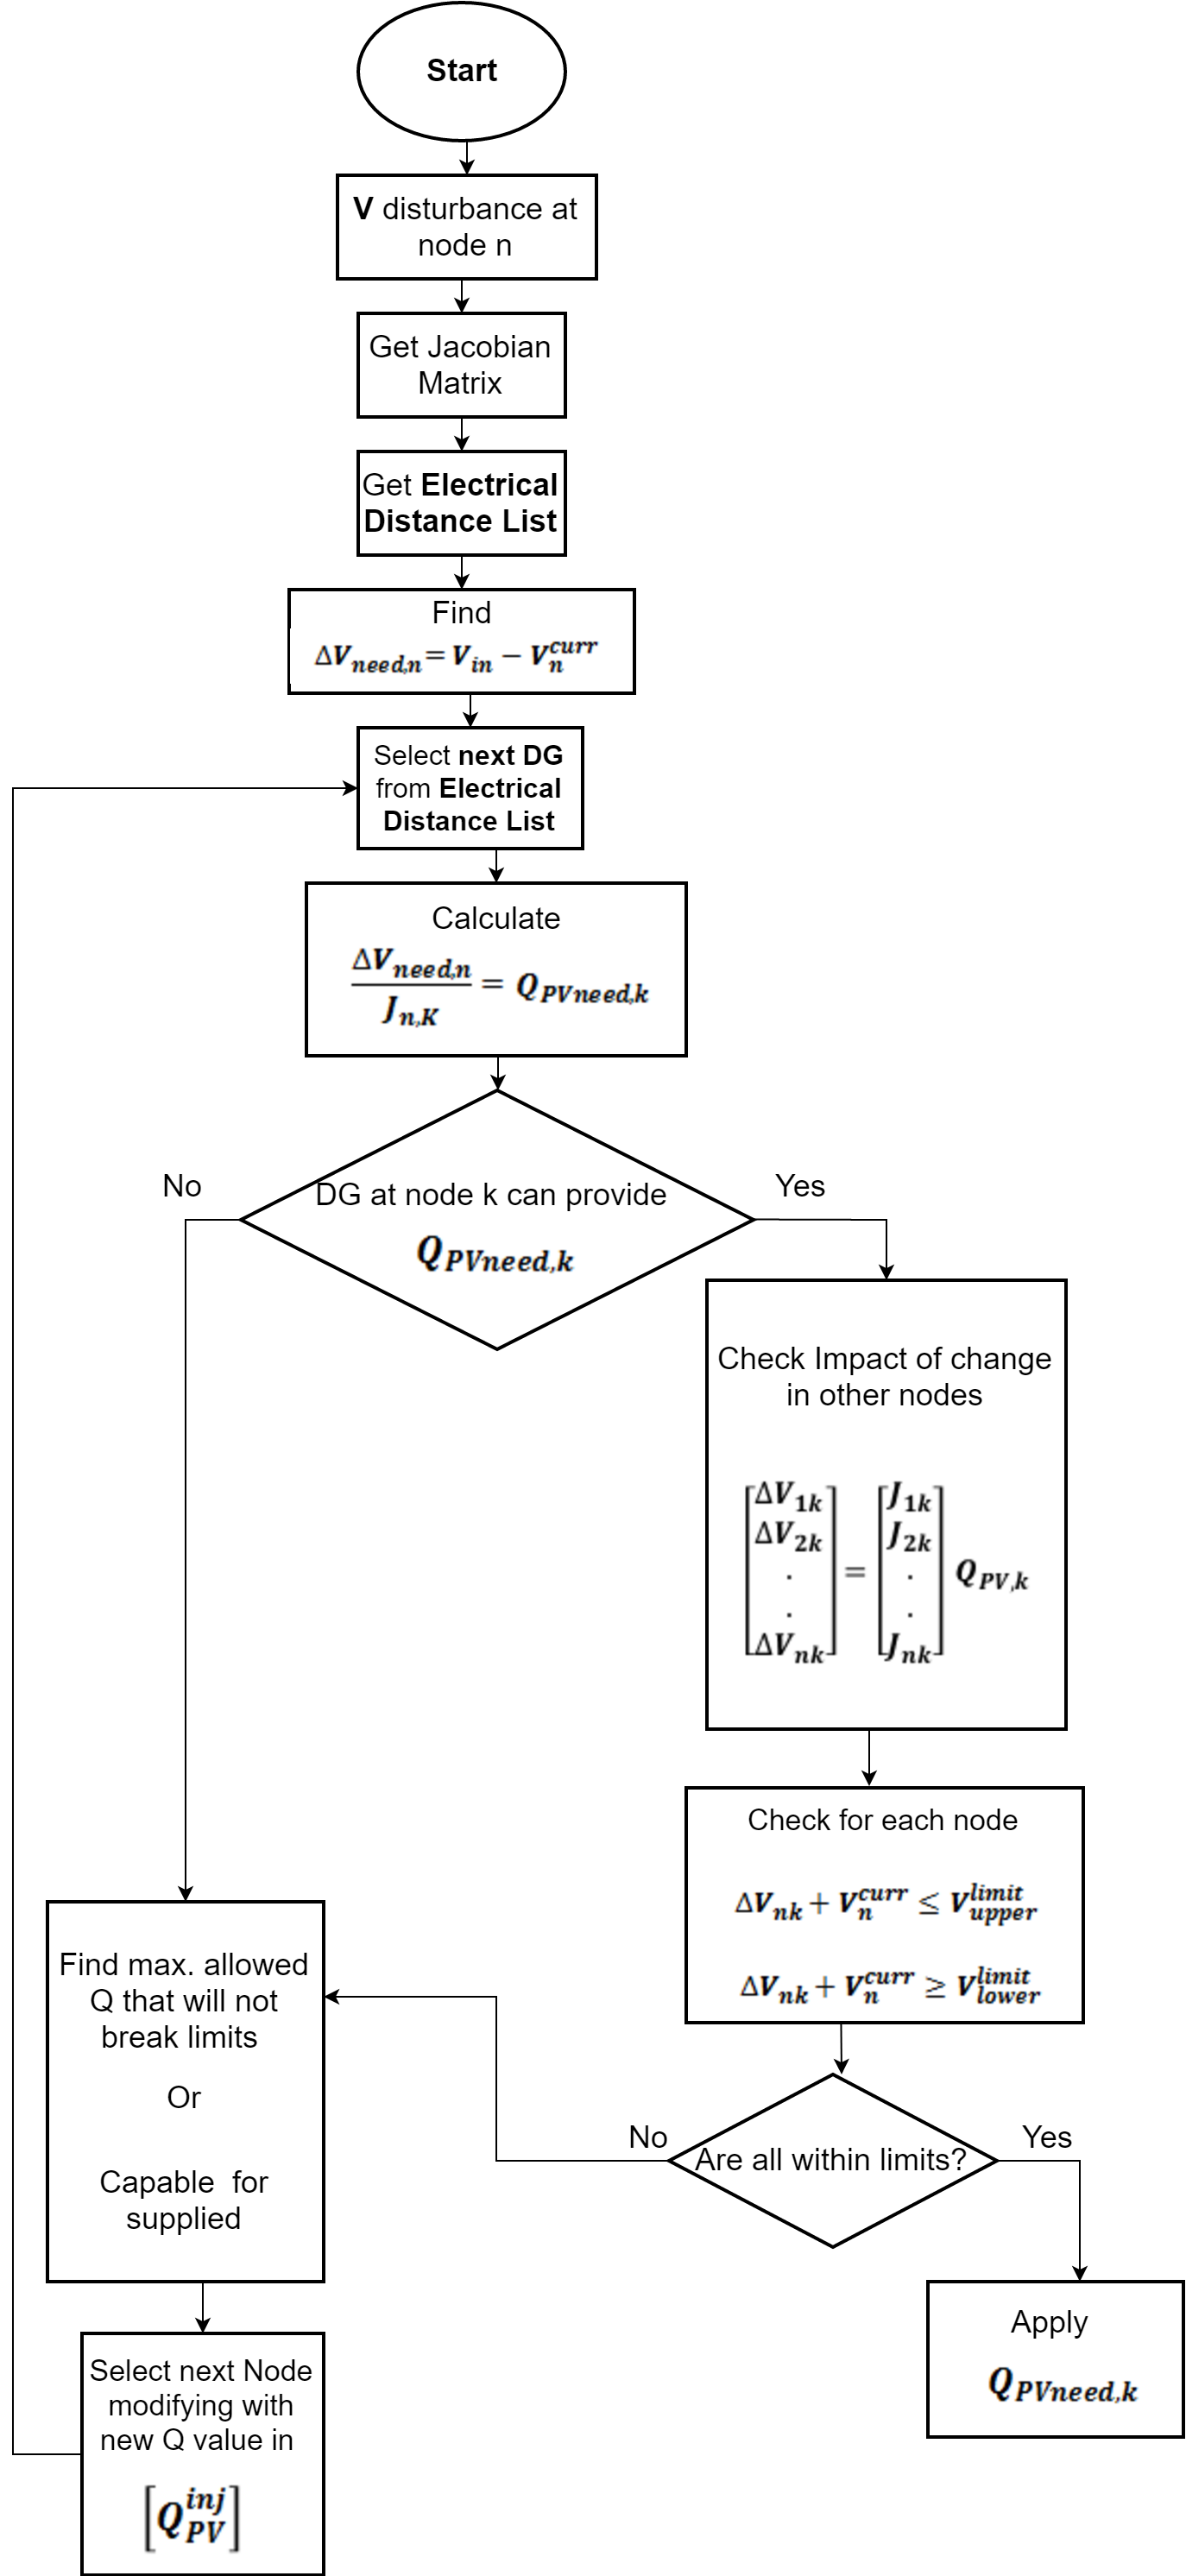
\includegraphics[width=0.5\textwidth]{cvc_alg.png}
% \caption{Coordinated Voltage Control Algorithm Flowchart}
% \label{fig:f1}
% \end{figure}
% The algorithm starts by receiving the needed information from the remote locations. It obtains the voltage and current measurements for each bus and the real and reactive power being generated or absorbed by the DGs. Based on these values, all the voltages are checked against the maximum and minimum voltage range criteria to detect under-voltage or over-voltage issues on specific nodes. When a voltage deviation is detected, the algorithm will start solving the issue from the furthest node to the closest one. The first step in solving this deviation is the application of voltage sensitivity concept to the affected node in order to find the approximate amount of reactive needed be injected at all nodes on control zone of the system. The voltage sensitivity process will return the Jacobian matrix for the system, Jvpq, and the reactive power that each node, in the control zone of the affected bus, needs to individually inject to solve the voltage deviation problem.  After this calculation is completed, a priority list of the nodes on control zone is created based on the criteria of the electrical distances calculated using the method mentioned above. The node closest to the affected node is selected and checked against the nodes that can inject reactive power into the system, in other words, the list of the nodes with DG connected to them. If the node selected to help in the voltage control has the capability of injecting reactive power, the value is checked against all other nodes to assure the compatibility of the value and make sure that no other voltage nodes get out of the desired bounds. As seen on the flowchart, if this value complies with the requirements mentioned, the reactive power reference value is sent to the respective DG inverter. If the value does not comply with the requirements, the next node in the electrical list is selected and the entire process is performed again. Another option for the solution of the reactive power reference calculation, is the application of the maximum reactive power that the current node can supply and the rerun of the entire algorithm to find the solution for the remaining voltage deviation. The algorithm is designed to handle both of these cases and try to minimize the impact in voltage caused by reactive power being injected or absorbed into the system. 




%\subsection{Test System}



\section{Test system}
The distribution network used for testing the coordinated voltage control algorithm is the test system number 2, available under the SUNGRIN project \cite{SG}. This test system was obtained by reducing the network of a larger feeder and it represents a real system in the state of Florida. Fig. \ref{fig:Feeder2} \cite{SG} depicts the topology of the network. The tests were performed considering a balanced system, making it a 9 bus test system. The data for the loads and the PV profiles were also obtained from the SUNGRIN project for that specific location. Fig. \ref{fig:pv_data} shows the real power generation of the three PVs present in the system. The used profile data has a resolution of one minute. Table \ref{tab:load_data} represents the rated values of the loads in the system. Table \ref{tab:Inv_rate} presents the rating of the inverters connected to the PV systems. The inverter reactive power limits (Q limits) are determined by considering a maximum of 0.8 power factor at the point of common coupling. 

\begin{figure}[!h]
\centering
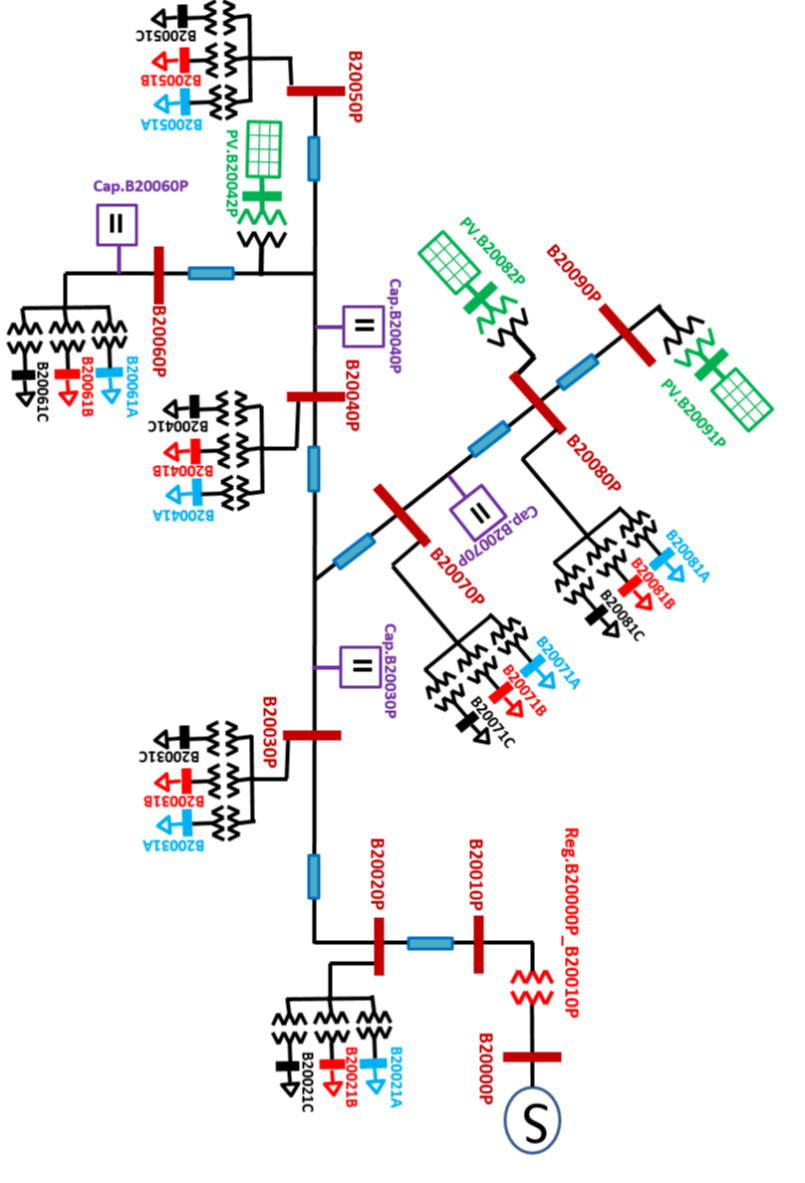
\includegraphics[width=\linewidth]{figs/feeder_r.png}
\caption{Test Feeder Topology.}
\label{fig:Feeder2}
\end{figure}

\begin{figure}[!h]
\centering
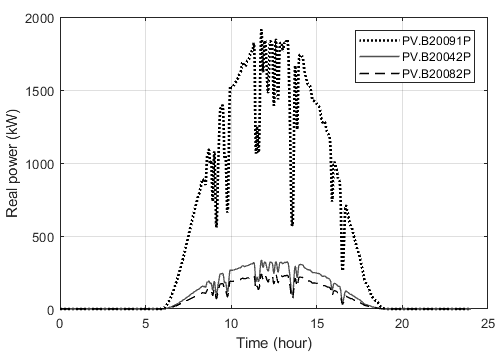
\includegraphics[width=\linewidth]{figs/PV_DATA.png}
\caption{Test Feeder Topology}
\label{fig:pv_data}
\end{figure}
% \begin{figure}[!h]
% \centering
% 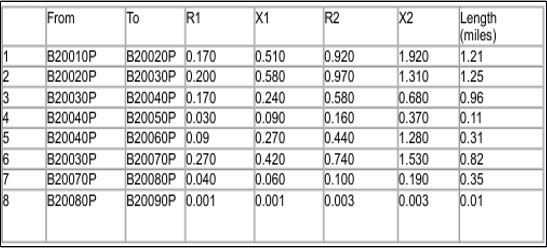
\includegraphics[width=7cm, height=3cm]{linedata.png}
% \caption{Line Data for the Distribution Network}
% \label{fig:BD1}
% \end{figure}

\begin{table}[!h]
\caption{Average load at nodes}
\label{tab:load_data}
\centering
\begin{tabular}{|c|c|c|}
\hline
Load & kVA & Power factor \\ \hline
B20020P & 1035 & 0.90 \\ \hline
B20030P & 2300 & 0.90 \\ \hline
B20040P & 1195 & 0.85 \\ \hline
B20050P & 225 & 0.85 \\ \hline
B20060P & 1285 & 0.85 \\ \hline
B20070P & 1365 & 0.85 \\ \hline
B20080P & 435 & 0.85 \\ \hline
\end{tabular}
\end{table}

% \begin{figure}[!h]
% \centering
% 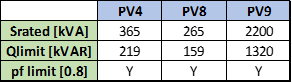
\includegraphics[width=6cm, height=2cm]{pvdata.png}
% \caption{PV Inverter Ratings}
% \label{fig:Inv_rate}
% \end{figure}

\begin{table}[!h]
\centering
\caption{PV Inverter Ratings}
\label{tab:Inv_rate}
\begin{tabular}{c|c|c|c|}
\cline{2-4}
 & PV.B20091P & PV.B20042P & PV.B20082P \\ \hline
\multicolumn{1}{|c|}{Rated power (kVA)} & 365 & 265 & 2200 \\ \hline
\multicolumn{1}{|c|}{Q limit (kVAR)} & 219 & 159 & 1320 \\ \hline
\end{tabular}
\end{table}

\section{Validation and Results}\label{sec:val}
A phasor model of the system shown in Fig. \ref{fig:Feeder2} is modeled and simulated  in MATLAB\textsuperscript{\textregistered} Simulink\textsuperscript{\textregistered} using the Simscape Power Systems\textsuperscript{TM} toolbox for validating the algorithm. Fig. \ref{fig:without_vvc} shows the per-unit feeder bus voltages for 86,400 seconds (24 hours) without implementing the control algorithm. The legends V1, V2, V3, V4, V5, V6, V7, V8 and V9 in the figure represent the per-unit (PU) voltages of buses B20010P, B20020P, B20030P, B20040P, B20050P, B20060P, B20070P, B20080P and B20090P respectively. As it can be seen in the figure, the bus voltages drop below the 0.95 PU limit  when the algorithm is not activated.

\begin{figure}[!h]
\centering
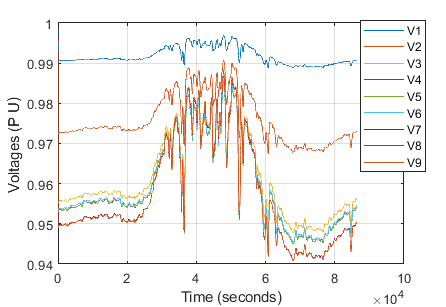
\includegraphics[width=\linewidth]{figs/Without_VVC.png}
\caption{Voltage Profile without Coordinated Voltage Control}
\label{fig:without_vvc}
\end{figure}

Fig. \ref{fig:with_cvc} presents the voltage profiles of all the nodes in the system with the coordinated voltage control activated. To show the effectiveness of the proposed algorithm the voltage bounds were set between 0.97 PU and 1.01 PU. It can be seen in the figure that the algorithm is capable of maintaining the voltages within the bounds by coordinating the DG inverters and capacitor banks available in the system. Fig. \ref{fig:DG_Q} shows the reactive power supplied by the DGs during the simulation. Fig \ref{fig:cap_bank} shows the switching states of capacitor banks Cap.B20040P, Cap.B20030P and Cap.B20070P. The capacitor bank Cap.B20060P is not used to regulate voltage because it is defined as always on in the system specification. The switching status 1 means that the capacitor bank is connected and the switching status 0 means that the capacitor bank is disconnected. It can be seen from the figures that the coordinated voltage control algorithm was able to maintain the system voltage status within the bounds mostly by using the DG inverters. It required two switching operations from the cap bank Cap.B20070P in addition to the DG inverters capability to maintain system voltage within 0.97 PU and 1.01 PU. It should be noted that during the full 24 hour simulation the on load tap changing transformer situated between buses B20010P and 20000P was not required to control the system voltage. From Fig. \ref{fig:with_cvc} it can also be inferred that the algorithm responds rapidly to voltage violations. In the actual simulation the algorithm always performed the required calculations under a second.

\begin{figure}[!h]
\centering
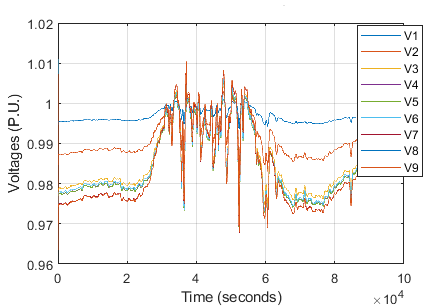
\includegraphics[width=\linewidth]{figs/With_VVC.png}
\caption{Voltage profile with coordinated voltage control}
\label{fig:with_cvc}
\end{figure}

\begin{figure}[!h]
\centering
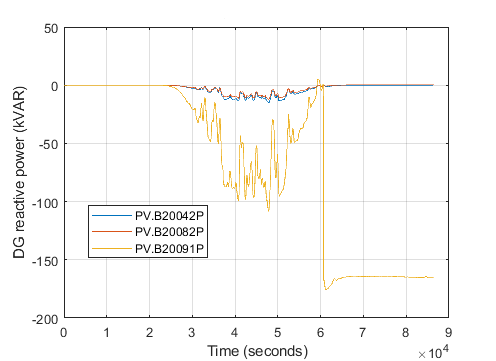
\includegraphics[width=\linewidth]{figs/DG_Q.png}
\caption{Reactive power supplied by DGs}
\label{fig:DG_Q}
\end{figure}

\begin{figure}[!h]
\centering
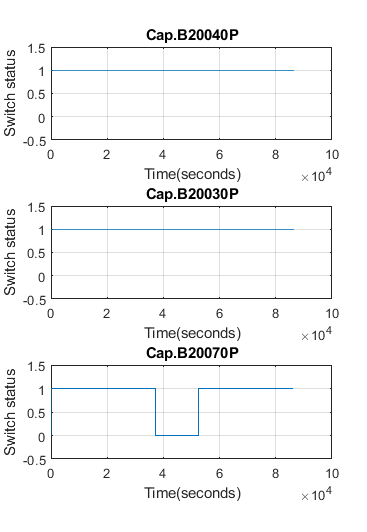
\includegraphics[width=\linewidth]{figs/CAP_BANK.png}
\caption{Capacitor bank switching states}
\label{fig:cap_bank}
\end{figure}


%\begin{enumerate}
%1
\item \textbf{Identify the nodes with voltage limit violation from measured data}
%2
\item \textbf{Determine node with highest voltage deviation.}
%3
\item \textbf{Construct system Jacobian matrix}
%4
\item \textbf{Calculate voltage sensitivity matrix}
%5
\item \textbf{Calculate electrical distances}
%6
\item \textbf{Order the nodes:} In this step, the nodes capable of providing reactive power support are ordered according to their electrical distance from the selected affected node. The ordered list of nodes is saved in a list called \textit{Node\_list}
%7
\item \textbf{Apply the appropriate reactive power:} In this step, the first node in the \textit{Node\_list} is selected. If the node has the capability to supply the required reactive power determined by the sensitivity matrix the algorithm sets the node to provide the required amount of power and continues to \textbf{step 9}. Otherwise, the algorithm sets the node to deliver the maximum available reactive power and takes it out of the list of nodes capable of providing reactive power.
%8
\item \textbf{Repeat steps 3 to 7}
%9
\item \textbf{Estimate new system status:} After deciding the change in node reactive powers the algorithm estimates the new voltage profile of the system using (\ref{eq.Q_V}). If all the nodes in the new estimated profile are within voltage limits the algorithm continues to \textbf{step 10}. Otherwise the algorithm updates the measured data collected from the system with the new estimates and goes back to  \textbf{step 1}.

%10
\item \textbf{Request the devices at the nodes to apply calculated changes}
\end{enumerate}

\section{Conclusion}
As the penetration of distributed generation resources starts to increase in distribution networks, the deployment of a coordinated voltage scheme is a requirement most utilities will have to fulfill. As observed, the algorithm proposed in this paper has the ability to coordinate the reactive power reference points for the distributed generation and traditional voltage regulation devices located along the feeder, taking into account their potential impacts on the entire system. By using this approach, a reduction in the use of traditional regulation devices can be achieved and the voltage profiles along the network can be controlled for the most part by just using the already existing DG inverters present on the network. In future work this concept of control will be expanded to unbalanced networks.

\bibliographystyle{IEEEtran}
\bibliography{mybib.bib}

%%%%%%%%%%%%%%%%%%%%%%%%%%%%%%%%%%%%%%%%%%%%%%%%%

% \begin{thebibliography}{1}

% \bibitem{int1}
% D.~Ranamuka, A.~P. Agalgaonkar and K.~M. Muttaqi, "Online Coordinated Voltage Control in Distribution Systems Subjected to Structural Changes and DG Availability,"\emph{ IEEE Transactions on Smart Grid}, vol. 7, no. 2, pp. 580-591, 2016. 
% \bibitem{int2}
% W.~Sheng, K.~-y. Liu and S. Cheng, "A Trust Region SQP Method for Coordinated Voltage Control in Smart Distribution Grid," \emph{IEEE Transactions on Smart Grid}, vol. 7, no. 1, pp. 381 - 391, 2016. 
% \bibitem{Th_ali}
% A.~Hariri, "Simulation Tools and Techniques for Analyzing the Impacts of Photovoltaic System Integration," Tallahassee Florida State University, 2017. 

% \bibitem{int4}
%  Paul Brucke Reactive Power Control in Utility-Scale PV, Solarprofessional.com, 2014. [Online]. Available: http://solarprofessional.com/articles/design-installation/reactive-power-control-in-utility-scale-pv/page/0/5. [Accessed: 24- Apr- 2017].

% \bibitem{SG}
% R. Meeker, M. Steurer and M. Faruque, "High penetration solar PV deployment sunshine state grid initiative (SUNGRIN)," Center for Advanced Power Systems, Tallahassee, 2015.

% \end{thebibliography}

%%%%%%%%%%%%%%%%%%%%%%%%%%%%%%%%%%%%%%%%%%%%%%%%%%%%%%%%%%

\end{document}